\documentclass[sigconf,natbib=true]{acmart}

\usepackage{booktabs}
\usepackage{multirow}
\usepackage{array}
\usepackage{tabularx}
\usepackage[table]{xcolor}
\usepackage{graphicx}
\usepackage{balance}
\usepackage{enumitem}
\usepackage{tikz}
\usetikzlibrary{arrows.meta, positioning, shapes.geometric, fit, backgrounds}

\graphicspath{{figures/}}

\setcopyright{none}
\settopmatter{printacmref=false, printccs=true, printfolios=true}
\renewcommand\footnotetextcopyrightpermission[1]{}

\acmConference[CIKM '26]{The 35th ACM International Conference on Information and Knowledge Management}{November 2026}{Rome, Italy}
\acmYear{2026}
\copyrightyear{2026}
\acmDOI{}
\acmISBN{}

\begin{document}

\title{RAG Under Extreme Data: System Design and Evaluation\\for Noisy Heterogeneous Institutional Corpora}

\author{[Author names redacted for review]}
\affiliation{\institution{[Institution redacted for review]}}

%%% ---------------------------------------------------------------
\begin{abstract}
Retrieval-augmented generation (RAG) chatbots are typically evaluated on clean, well-structured corpora with high-quality benchmarks.
Institutional deployments face two compounding problems that together make evaluation fundamentally unreliable.
First, the knowledge base is built from \emph{extremely noisy, heterogeneous} sources: faculty web pages whose HTML structure is inconsistent even within the same CMS, dynamically generated timetable pages that use incompatible table structures across different course groups, PDFs behind authentication walls that resist automated access, and Excel files whose relational cell meaning evaporates on flattening.
These are not edge cases---they are the typical state of institutional data, and no chunking strategy designed for Wikipedia or news articles survives contact with them.
Second, the evaluation data itself is unreliable: ad hoc student survey questions are too short (mean 6.8 words), terse, and poorly annotated to constitute a valid benchmark---a direct consequence of collecting queries from users who were not asked to formulate realistic test cases.

We present MiNIonek, a deployed end-to-end RAG chatbot for a Polish technical university faculty, and describe a systematic response to both problems.
For the knowledge base problem, we use \emph{atomic fact extraction}: GPT-4o-mini decomposes each source document into self-contained factual statements before embedding and indexing, making the representation noise-tolerant by design.
For the evaluation quality problem, we construct a \emph{synthetic query set} of 1{,}428 questions generated by NotebookLM with direct access to the full knowledge base---well-formed queries with verified source citations at near-zero annotation cost.

We conduct a five-variant off-line ablation study across hybrid vs.\ dense-only retrieval, one- and two-step re-ranking, and LLM-based query rewriting, evaluated at both extremes of the query quality spectrum.
Fact extraction improves retrieval precision on synthetic queries (Hit@1 +7.3\,pp, MRR@5 +4.5\,pp) while chunk-based retrieval dominates on ad hoc queries (Hit@5 +22.7\,pp).
Query rewriting \emph{hurts} retrieval on ad hoc queries by 13.4\,pp Hit@5.
LLM judge scores are 1.27 points higher on structured synthetic questions than on terse ad hoc queries under identical pipeline conditions---demonstrating that judge calibration depends on query distribution, a systematic risk in off-line evaluation.
The deployed chatbot scored 9.2\,/\,10.0 in a five-day live user study with 14 student evaluators.
\end{abstract}

\begin{CCSXML}
<ccs2012>
 <concept>
  <concept_id>10002951.10003317.10003347.10003350</concept_id>
  <concept_desc>Information systems~Retrieval models and ranking</concept_desc>
  <concept_significance>500</concept_significance>
 </concept>
 <concept>
  <concept_id>10002951.10003317.10003331.10003333</concept_id>
  <concept_desc>Information systems~Question answering</concept_desc>
  <concept_significance>500</concept_significance>
 </concept>
 <concept>
  <concept_id>10002951.10003317.10003334.10003342</concept_id>
  <concept_desc>Information systems~Evaluation of retrieval results</concept_desc>
  <concept_significance>300</concept_significance>
 </concept>
 <concept>
  <concept_id>10002951.10003317.10003347.10003351</concept_id>
  <concept_desc>Information systems~Query reformulation</concept_desc>
  <concept_significance>300</concept_significance>
 </concept>
 <concept>
  <concept_id>10002951.10003317.10003349.10003352</concept_id>
  <concept_desc>Information systems~Specialized information retrieval</concept_desc>
  <concept_significance>300</concept_significance>
 </concept>
</ccs2012>
\end{CCSXML}

\ccsdesc[500]{Information systems~Retrieval models and ranking}
\ccsdesc[500]{Information systems~Question answering}
\ccsdesc[300]{Information systems~Evaluation of retrieval results}
\ccsdesc[300]{Information systems~Query reformulation}
\ccsdesc[300]{Information systems~Specialized information retrieval}

\keywords{retrieval-augmented generation, chatbot, end-to-end pipeline, atomic fact extraction, hybrid retrieval, extremely noisy corpora, off-line evaluation, ad hoc queries, synthetic test set, LLM-as-a-judge, ablation study}

\maketitle

%%% ---------------------------------------------------------------
\section{Introduction}
\label{sec:intro}
%%% ---------------------------------------------------------------

Retrieval-augmented generation (RAG)~\cite{lewis2020rag,gao2023rag_survey} augments language models with an external document store, enabling question answering over knowledge that exceeds parametric capacity.
Most published RAG research assumes the central challenge is retrieval or generation---and evaluates systems against carefully curated corpora with high-quality annotated benchmarks~\cite{es2023ragas,yu2024ragsurvey}.
For institutional deployments, neither assumption holds.

Consider a faculty chatbot whose knowledge base is assembled from the institution's actual digital footprint: faculty web pages in which the same CMS template renders inconsistently across departments; timetable pages dynamically generated by the student registry system, using incompatible HTML table structures for different course groups, some with \texttt{rowspan}-encoded multi-hour slots that become invisible after flattening, others with repeated cells, others omitting the building identifier entirely; PDF documents behind faculty login pages that block all automated access; and Excel schedule files whose time-slot--course--room meaning evaporates when the spreadsheet is read as flat text.
These are not edge cases---they are the \emph{typical} state of institutional data.
The key observation is that this is not primarily a scraping problem: Firecrawl returns valid Markdown for all accessible pages.
The problem is that the \emph{source HTML is itself ill-structured and inconsistent at its origin}, and no scraper improvement can correct data that was never consistently authored.

The evaluation data presents a symmetrical challenge.
Student survey questions collected ad hoc are short (mean 6.8 words), terse, and imprecisely annotated---not because students are careless, but because a survey form does not motivate precise, realistic questions.
51\% of collected questions have no grounding document in the corpus at all: students asked about university-wide regulations, individual academic records, or personal matters that a faculty chatbot cannot answer.
Measuring a system against this benchmark yields misleading scores and does not predict live user satisfaction.

We address both challenges in the context of MiNIonek, a deployed end-to-end RAG chatbot for the Faculty of Mathematics and Information Science (MiNI) at Warsaw University of Technology.
Our response to the data quality problem is \emph{atomic fact extraction}: before embedding, every source document is processed by a language model that decomposes it into a list of self-contained factual statements.
This eliminates arbitrary chunking boundaries, removes format noise, and produces compact retrieval units that are individually interpretable---noise-tolerant because the model must \emph{understand and paraphrase}, not copy.
Our response to the evaluation quality problem is \emph{synthetic query generation}: NotebookLM, supplied with the full knowledge base, generates 1{,}428 questions with verified source citations, approximating the complex multi-entity queries that real users ask when they have a genuine information need.

We frame the evaluation as \emph{extreme evaluation}: we test the system at both ends of the query quality spectrum---ad hoc queries that are maximally short and noisy (lower bound), and synthetic queries that are maximally well-formed and precisely annotated (upper bound).
Real student usage falls between these extremes and is substantially closer to the synthetic end when users have a genuine, complex question.
The gap between the two distributions is itself an empirical finding with practical implications: a system optimised on ad hoc queries will systematically underperform on real complex usage.

\smallskip\noindent Our contributions are:
\begin{enumerate}[label=(\roman*),topsep=2pt,itemsep=0pt]
  \item a characterisation of the structural failure modes of extremely noisy, heterogeneous institutional corpora and why standard RAG chunking fails on them;
  \item an end-to-end atomic fact extraction pipeline that simultaneously solves the chunking boundary problem and removes format noise across five heterogeneous source types;
  \item a procedure for generating high-quality synthetic evaluation sets via a retrieval-augmented generator, applicable when ad hoc benchmarks are too noisy to serve as reliable signals;
  \item a five-variant off-line ablation study with block-level pipeline analysis across both ad hoc and synthetic query distributions;
  \item an empirical demonstration that LLM judge scores depend on query distribution, with implications for off-line evaluation reliability.
\end{enumerate}

%%% ---------------------------------------------------------------
\section{Related Work}
%%% ---------------------------------------------------------------

\paragraph{RAG architectures.}
The foundational RAG architecture~\cite{lewis2020rag} retrieves documents using dense retrieval~\cite{karpukhin2020dpr} and conditions generation on the concatenated evidence.
Subsequent work has refined the pipeline: FLARE~\cite{jiang2023flare} retrieves iteratively; Self-RAG~\cite{asai2023selfrag} adds retrieval and critique tokens; adaptive retrieval~\cite{mallen2023trust} decides whether to retrieve at all.
Our study does not modify the high-level architecture but targets the pre-retrieval data preparation stage, which is underexplored relative to the attention given to retrieval and generation.

\paragraph{Chunking strategies.}
Standard chunking approaches include fixed-size sliding windows, sentence-level splits, and semantic chunking~\cite{shi2023chunking}.
Proposition indexing~\cite{chen2023densex} is the closest prior work: it uses an LLM to decompose passages into atomic propositions before indexing.
We independently arrive at a similar strategy, extend it to a heterogeneous multi-format corpus, and evaluate it in a deployed system against both precision-oriented and recall-oriented query distributions.

\paragraph{Hybrid retrieval and re-ranking.}
BM25~\cite{robertson2009bm25} and dense retrieval are complementary: dense retrieval generalises across vocabulary, sparse retrieval is precise on named entities.
RRF~\cite{cormack2009rrf} fuses both ranked lists without score normalisation.
Cross-encoder re-ranking~\cite{nogueira2019passage} refines the retrieved shortlist with full query--passage attention.
We contribute an ablation showing that both techniques are query-distribution-dependent: BM25 and re-ranking benefit long structured queries but add little value on short ad hoc ones.

\paragraph{Query transformation.}
HyDE~\cite{gao2023hyde} expands the query into a hypothetical answer; Query2Doc~\cite{wang2023query2doc} adds generated context.
We use a simpler variant: a low-temperature LLM rewrite that expands short queries into keyword-rich form.
We find---unexpectedly---that this \emph{hurts} retrieval on ad hoc queries, reversing the standard recommendation.

\paragraph{LLM as a judge.}
Zheng et al.~\cite{zheng2023judging} establish GPT-4 as a reliable judge for open-ended quality.
RAGAS~\cite{es2023ragas} adapts this to RAG evaluation.
Pan et al.~\cite{pan2024llmjudge} study systematic biases including length and verbosity preference.
We add a new bias: judges score the same system substantially higher on well-formed synthetic questions than on short ad hoc ones under identical pipeline conditions---a \emph{query-distribution bias} that is especially dangerous in off-line evaluation.

\paragraph{Evaluation on real vs.\ synthetic queries.}
The companion paper~\cite{[COMPANION_PAPER]} characterises the distributional gap between synthetic and production queries along four dimensions and reports a 37\,pp Hit@5 gap.
We build on this infrastructure to study which pipeline components close the gap most efficiently.

%%% ---------------------------------------------------------------
\section{Corpus and Extreme Data Challenges}
\label{sec:corpus}
%%% ---------------------------------------------------------------

The MiNI faculty information corpus is assembled from five source types:

\begin{itemize}[topsep=2pt,itemsep=0pt]
  \item \textbf{Web pages}: over 300 URLs from the faculty website, scraped via Firecrawl~\cite{firecrawl} and returned as HTML-to-Markdown. Layouts vary widely and inconsistently within the same site.
  \item \textbf{PDFs}: 18 documents from the institutional information bulletin (BIP), requiring a faculty login and therefore downloaded manually. Includes official regulations, scholarship thresholds, and examination rules.
  \item \textbf{XLSX and DOCX files}: structured documents including timetable spreadsheets and Word procedure tables, pre-processed to plain text before ingestion.
  \item \textbf{USOS schedule pages}: dynamically generated timetable pages from the university registration system, parsed via a dedicated custom scraper that preserves time-slot--course--room structure.
  \item \textbf{Static facts}: 7 high-traffic facts (dean's name, office address, main URL) injected directly into the system prompt at inference time.
\end{itemize}

\subsection{Why Standard Pipelines Break}

We identify four data quality failures that are pervasive across all source types and defeat standard RAG ingestion.

\textbf{Inconsistent HTML structure.}
The faculty website is served from a CMS that renders the same template differently for different departments and page types.
Navigation menus, footer links, and breadcrumb trails are included in the scraped Markdown alongside body text, because the HTML does not use semantic sectioning tags consistently.
The same information (e.g.\ scholarship deadlines) may appear on three pages with three different Markdown structures: a heading-list on one, a prose paragraph on another, and a table on a third.
A fixed chunking window captures fundamentally different content depending on which page variant it encounters.

\textbf{Schedule page fragmentation and inconsistency.}
USOS timetable pages are generated dynamically and share a common URL pattern but differ in HTML table structure across course groups in ways that cannot be predicted from the URL.
Some course groups encode multi-hour time slots using \texttt{rowspan} attributes that become invisible after flattening; others repeat cells; some omit the building identifier; some use numeric HTML character references for Polish diacritics while others use UTF-8 directly; some group entries by day while others sort by time.
A 512-token chunk extracted from these pages may contain 20--30 course slots from different days in a sequence that reflects neither the weekly timetable structure nor any consistent sort order.
The correct fact---\textit{``Group A2 of Year-2 Computer Science attends Linear Algebra on Tuesdays from 10:15 to 12:00 in room 318, building MiNI''}---does not survive any fixed-window chunking strategy applied to this layout.

\textbf{PDF encoding artefacts.}
PDF text extraction introduces hyphenation at arbitrary line boundaries, garbled Polish diacritics where the embedded font does not map correctly to Unicode, and lost whitespace from multi-column layouts.
Table cells from regulation documents are extracted as contiguous text streams with no structural markers.

\textbf{Cross-format duplication and stale content.}
The same information frequently exists in multiple formats: a regulation as both a PDF and a web rendering; a timetable as both USOS pages and a downloadable XLSX.
These duplicates use different vocabulary and formatting, causing the same underlying fact to appear in the index multiple times with different retrieval characteristics.
This also creates false negatives in URL-based evaluation: the system may retrieve the correct fact from the XLSX version when the evaluation gold annotation points to the USOS page.

\subsection{Why Better Scraping Alone Is Not the Answer}

A key observation is that Firecrawl returns valid Markdown for all pages it can access.
The problem is that the \emph{source HTML is itself ill-formed and inconsistently structured at its origin}: timetable inconsistencies between course groups reflect actual inconsistencies in how data was entered into the registry system, not a rendering bug; PDF encoding errors are present in the source files; navigation artefacts exist in the page HTML.
No scraper improvement corrects data that was never consistently authored.

This motivates our central response: rather than trying to chunk and index raw noisy source text, we use a language model to \emph{understand and paraphrase}.
Fact extraction is noise-tolerant by design---the model reads garbled hyphenations, disambiguates implicit subjects, and resolves pronoun coreference before producing the indexed text.

%%% ---------------------------------------------------------------
\section{System Architecture}
\label{sec:architecture}
%%% ---------------------------------------------------------------

Figure~\ref{fig:architecture} shows the end-to-end pipeline.
We use labels \textbf{[I1]--[I6]} for the offline ingestion path and \textbf{[R1]--[R8]} for the online inference path; block labels are referenced throughout the ablation study (Section~\ref{sec:variants}).

\begin{figure}[t]
\centering
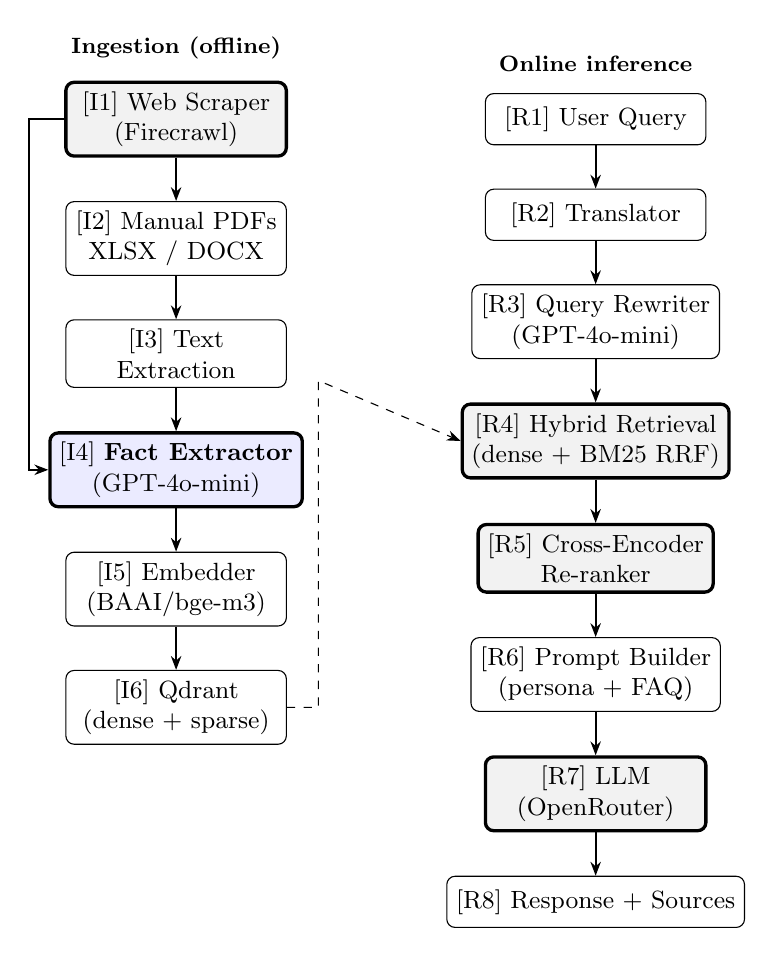
\begin{tikzpicture}[
    font=\small,
    box/.style={draw, rounded corners=3pt, minimum width=2.8cm,
                minimum height=0.65cm, align=center, fill=white},
    boldbox/.style={box, line width=1.2pt, fill=gray!10},
    arr/.style={-{Stealth[length=5pt]}, thick},
    dasharr/.style={-{Stealth[length=5pt]}, dashed, thin},
    node distance=0.55cm and 1.1cm
]

%% ---- INGESTION (left column) -----------------------------------
\node[boldbox] (scraper)  {[I1] Web Scraper\\(Firecrawl)};
\node[box, below=of scraper] (pdfs)    {[I2] Manual PDFs\\XLSX / DOCX};
\node[box, below=of pdfs]    (proc)    {[I3] Text\\Extraction};
\node[boldbox, below=of proc, fill=blue!8] (facts) {[I4] \textbf{Fact Extractor}\\(GPT-4o-mini)};
\node[box, below=of facts]   (embed)   {[I5] Embedder\\(BAAI/bge-m3)};
\node[box, below=of embed]   (qdrant)  {[I6] Qdrant\\(dense + sparse)};

\draw[arr] (scraper) -- (pdfs);
\draw[arr] (pdfs)    -- (proc);
\draw[arr] (proc)    -- (facts);
\draw[arr] (facts)   -- (embed);
\draw[arr] (embed)   -- (qdrant);

%% ---- ONLINE (right column) -------------------------------------
\node[box, right=2.5cm of scraper]  (user)   {[R1] User Query};
\node[box, below=of user]           (trans)  {[R2] Translator};
\node[box, below=of trans]          (rewrite){[R3] Query Rewriter\\(GPT-4o-mini)};
\node[boldbox, below=of rewrite]    (hybrid) {[R4] Hybrid Retrieval\\(dense + BM25 RRF)};
\node[boldbox, below=of hybrid]     (rerank) {[R5] Cross-Encoder\\Re-ranker};
\node[box, below=of rerank]         (prompt) {[R6] Prompt Builder\\(persona + FAQ)};
\node[boldbox, below=of prompt]     (llm)    {[R7] LLM\\(OpenRouter)};
\node[box, below=of llm]            (out)    {[R8] Response + Sources};

\draw[arr] (user)    -- (trans);
\draw[arr] (trans)   -- (rewrite);
\draw[arr] (rewrite) -- (hybrid);
\draw[arr] (hybrid)  -- (rerank);
\draw[arr] (rerank)  -- (prompt);
\draw[arr] (prompt)  -- (llm);
\draw[arr] (llm)     -- (out);

\draw[arr] (scraper.west) -- ++(-0.45,0) |- (facts.west);
\draw[dasharr] (qdrant.east) -- ++(0.4,0) -- ++(0, 4.15) -- (hybrid.west);

\node[above=0.15cm of scraper, font=\footnotesize\bfseries] {Ingestion (offline)};
\node[above=0.15cm of user,    font=\footnotesize\bfseries] {Online inference};

\end{tikzpicture}
\caption{MiNIonek end-to-end pipeline. Block labels [I1]--[I6] (ingestion) and [R1]--[R8] (online inference) are referenced in the ablation study. Bold boxes are components varied across ablation variants. \textbf{[I4]} is the primary response to the data quality problem; \textbf{[R3]}, \textbf{[R4]}, and \textbf{[R5]} are the retrieval components studied in the ablation.}
\label{fig:architecture}
\end{figure}

\subsection{Ingestion Components [I1]--[I6]}

\textbf{[I1] Web Scraper.}
Firecrawl~\cite{firecrawl} converts faculty web pages to Markdown.
For USOS schedule pages, a dedicated custom scraper (Python \texttt{requests} + BeautifulSoup) is used instead, to preserve the time-slot--course--room structure that generic HTML-to-Markdown conversion loses when collapsing \texttt{rowspan}/\texttt{colspan} attributes.

\textbf{[I2] Manual Document Sources.}
PDFs requiring faculty authentication, XLSX timetable files, and DOCX procedure documents are downloaded manually and pre-processed: PDFs via \texttt{pdfminer}, XLSX via \texttt{openpyxl} with cell-by-cell extraction preserving row--column position, DOCX via \texttt{python-docx}.

\textbf{[I3] Text Extraction \& Normalisation.}
Raw extracted text undergoes normalisation: common Polish diacritic encoding errors are corrected, navigation artefacts (breadcrumbs, cookie banners, ``skip to content'' links) are removed, and excessive whitespace is collapsed.

\textbf{[I4] Atomic Fact Extractor.}
The core response to the data quality problem.
GPT-4o-mini is prompted to enumerate \emph{every} verifiable statement in the source text as an independent, fully self-contained sentence with no pronoun coreference and no implicit subject.
The extraction prompt explicitly prohibits selective filtering for ``importance'': without this constraint, models suppress office hours, room numbers, and administrative deadlines---exactly the facts students most commonly query.
Each extracted fact is stored as a separate Qdrant point with the source URL as metadata.
The full knowledge base contains 36{,}585 atomic facts; the 36-source evaluation subset contains 11{,}407 facts.

A fact extracted from a USOS schedule entry reads: \textit{``The Linear Algebra lecture for Group A1 of Year-1 Computer Science meets every Monday from 10:15 to 12:00 in room 318, building MiNI, taught by [Instructor].''} This is fully retrievable for any named entity in the sentence. A raw 512-token chunk from the same page contains 20--30 such slots for unrelated course groups, diluting the retrieval signal for any single query.

\textbf{[I5] Embedder.}
BAAI/bge-m3~\cite{xiao2024bge} produces 1024-dimensional dense vectors.
It is a state-of-the-art multilingual model supporting Polish, English, and Ukrainian---all three languages in the faculty's student body.
Sparse BM25-compatible vectors are produced via the bge-m3 sparse variant through FastEmbed.

\textbf{[I6] Qdrant Vector Store.}
Dense and sparse vectors are stored in separate Qdrant collections, enabling hybrid or dense-only retrieval at query time without re-indexing.

\subsection{Online Inference Components [R1]--[R8]}

\textbf{[R1] User Query.}
The React/Vite frontend collects the user's question together with a user-type selection: junior/senior undergraduate, master's, doctoral, prospective student, administrative staff, or research staff. The user type is forwarded to [R6] for persona injection.

\textbf{[R2] Translator.}
A language detector checks whether the query is in Polish. Non-Polish queries (English or Ukrainian) are translated to Polish before retrieval, since the knowledge base is Polish-language. Generated responses are translated back to the user's detected language.

\textbf{[R3] Query Rewriter.}
GPT-4o-mini (temperature~0.0) rewrites the user's natural-language question into a keyword-rich retrieval query: colloquial phrasing is replaced with domain-specific Polish terminology.
For example, \textit{``kiedy mam zajęcia?''} (``when do I have class?'') becomes \textit{``plan zajęć harmonogram sala semestr termin WMiNI''}.
\textbf{This component is skipped in variant V5} (no-rewrite ablation).

\textbf{[R4] Hybrid Retrieval.}
Queries both the dense and sparse Qdrant collections using bge-m3 for dense encoding and the BM25 sparse model.
Each pre-fetch retrieves $3\times$ the target number of candidates (total: 180); Qdrant's built-in RRF~\cite{cormack2009rrf} fuses the two ranked lists and returns the top 60.
\textbf{In V2 (Dense-only)}, the sparse BM25 pre-fetch is disabled and dense retrieval alone returns the top 60.

\textbf{[R5] Cross-Encoder Re-ranker.}
A multilingual cross-encoder (\texttt{mmarco-mMiniLMv2-L12-H384-v1}) scores all 60 candidates jointly with the query using full cross-attention.
\textbf{In V1 (Baseline)}: one-step, $60 \to 30$.
\textbf{In V3 (No re-ranking)}: [R5] is skipped entirely and [R4] output passes directly to [R6].
\textbf{In V4 (Two-step)}: cascade $60 \to 30 \to 15$, applying the same cross-encoder to the 30 survivors.

\textbf{[R6] Prompt Builder.}
Assembles the system prompt from four components: (i)~role and rules (assistant name MiNIonek, priority ordering retrieved context $\succ$ static FAQ $\succ$ parametric knowledge, exhaustive-schedule rule); (ii)~persona based on the user-type selection from [R1]; (iii)~a static FAQ of 7 high-traffic facts that are both frequently queried and unlikely to change; (iv)~the top-30 facts from [R5], each delimited and tagged with their source URL. Conversation history is appended as alternating \texttt{user}/\texttt{assistant} message pairs.

\textbf{[R7] LLM Generator.}
GPT-4o-mini via OpenRouter generates the response. For users who attach a PDF document, the file is encoded as base64 and sent as a vision content block to multimodal-capable models (GPT-4o, Gemini~2.5 Flash).

\textbf{[R8] Response + Sources.}
The frontend renders the response with clickable source links parsed from Markdown-style \texttt{[text](url)} patterns and bare URLs.

%%% ---------------------------------------------------------------
\section{Evaluation Methodology}
\label{sec:eval}
%%% ---------------------------------------------------------------

\subsection{Off-line Evaluation Design}

Figure~\ref{fig:eval_design} illustrates the three-stage off-line evaluation design.
At each stage, one dimension is independently varied.
Tables in Section~\ref{sec:results} report results for specific combinations of (ingestion strategy, retrieval variant, query distribution).

\begin{figure}[h]
\centering
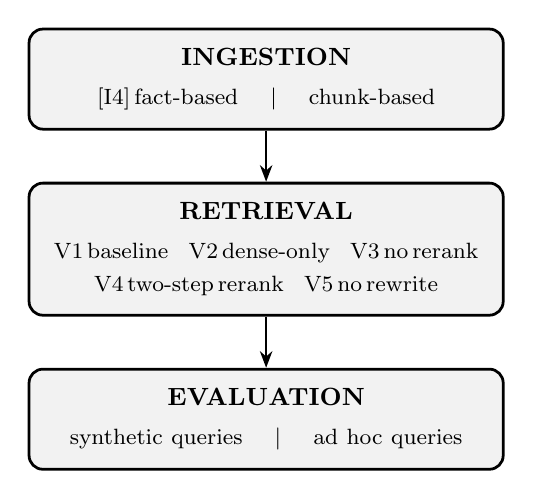
\begin{tikzpicture}[
  font=\small,
  mainblock/.style={draw, rounded corners=5pt, text width=5.6cm,
                    align=center, fill=gray!10, line width=1pt,
                    inner ysep=7pt, inner xsep=6pt},
  arr/.style={-{Stealth[length=6pt]}, thick},
  node distance=0.65cm
]

\node[mainblock] (ing) {
  \textbf{INGESTION}\\[3pt]
  {\footnotesize [I4]\,fact-based \quad $|$ \quad chunk-based}
};

\node[mainblock, below=of ing] (ret) {
  \textbf{RETRIEVAL}\\[3pt]
  {\footnotesize V1\,baseline \enspace V2\,dense-only \enspace V3\,no\,rerank}\\[1pt]
  {\footnotesize V4\,two-step\,rerank \enspace V5\,no\,rewrite}
};

\node[mainblock, below=of ret] (ev) {
  \textbf{EVALUATION}\\[3pt]
  {\footnotesize synthetic queries \quad $|$ \quad ad hoc queries}
};

\draw[arr] (ing) -- (ret);
\draw[arr] (ret) -- (ev);

\end{tikzpicture}
\caption{Off-line evaluation design. Each stage introduces independent variation: ingestion strategy (Tables~\ref{tab:facts_vs_chunks} and~\ref{tab:schedule_eval}), retrieval configuration (Table~\ref{tab:ablation}), and query distribution (all tables, two columns each).}
\label{fig:eval_design}
\end{figure}

\noindent The design directly reflects the two-problem framing of this paper.
\textbf{Ingestion-stage variation} (fact-based vs.\ chunk-based at [I4]) addresses the data quality problem.
\textbf{Evaluation-stage variation} (synthetic vs.\ ad hoc query distribution) addresses the benchmark quality problem.
Retrieval-stage variation (V1--V5) is studied with fixed fact-based ingestion and is evaluated against both query distributions to measure interaction effects.

\subsection{Query Sets: Ad Hoc vs.\ Synthetic}
\label{sec:querysets}

We use two query distributions that represent the extremes of the evaluation quality spectrum.

\paragraph{Ad hoc queries (real student survey).}
322 questions were collected by members of the faculty student science club via a structured survey.
These are \emph{ad hoc} queries: questions formulated by students on the spot, without guidance to produce realistic or complex test cases.
Their distributional properties reflect this origin:
mean question length of 6.8 words; 51\% lacking any grounding document in the corpus (students asked about university-wide regulations, personal academic records, and topics outside the corpus scope); gold URL annotations assigned by student volunteers without a formal annotation protocol, frequently pointing to parent pages rather than the specific sub-page containing the answer.
After filtering to questions with a confirmed gold URL present in the corpus, 165 questions remain for retrieval evaluation; 75 remain for the evaluation subset.

Representative examples: \textit{``kiedy dziekanat?''} (``when is the dean's office open?'', 2 words); \textit{``konsultacje prof.\ X''} (``professor X's office hours'', 3 words).

These queries constitute an \emph{extreme lower bound}: maximally short, maximally noisy, and imprecisely annotated.
A system that scores well against them has cleared a low bar.

\paragraph{Synthetic queries (NotebookLM).}
1{,}428 questions were generated by NotebookLM~\cite{notebooklm2024} supplied with the full knowledge base.
NotebookLM generates questions grounded in the provided sources, with paired reference answers and explicit source document citations---requiring no human annotation effort beyond spot-checking.
Their properties: mean question length of 15.7 words; all questions have a verified source citation; questions cover complex, multi-entity scenarios reflecting realistic student information needs.

Representative examples: \textit{``W jakich godzinach czynny jest dziekanat WMiNI i jaka jest procedura składania podania o urlop dziekański?''} (``What are the WMiNI dean's office hours and what is the procedure for applying for a dean's leave of absence?'', 20 words); \textit{``Kiedy odbywają się laboratoria z Analizy Danych dla grupy A2 i w jakiej sali?''} (``When are the Data Analysis labs for group A2 and in which room?'', 14 words).

\begin{table}[h]
\centering
\caption{Query set properties. ``Subset eval'' = questions with gold URL confirmed in the 36-source evaluation subset.}
\label{tab:querysets}
\small
\setlength{\tabcolsep}{4pt}
\begin{tabular}{lcc}
\toprule
\textbf{Property} & \textbf{Ad hoc} & \textbf{Synthetic} \\
\midrule
Total questions & 322 & 1{,}428 \\
Mean length (words) & 6.8 & 15.7 \\
Questions with gold URL & 165 & 1{,}428 \\
Subset eval questions & 75 & 1{,}041 \\
Source annotation & volunteer & auto (spot-checked) \\
Questions w/o corpus grounding & 51\% & ${<}1\%$ \\
\bottomrule
\end{tabular}
\end{table}

\paragraph{The two distributions as extreme evaluation bounds.}
We deliberately test at both extremes rather than a single query set.
Ad hoc queries represent the worst case: a survey instrument not designed to elicit realistic test cases.
Synthetic queries represent the best case: well-formed, precisely annotated questions that match the structure of information in the knowledge base.
Real student usage falls between these bounds and is substantially closer to the synthetic end when users have a genuine, complex information need.
A system optimised on ad hoc queries alone may appear to underperform on real-world complex usage; a system tested only on synthetic queries overestimates performance on terse everyday questions.
Testing at both extremes bounds the performance space and makes the interaction between pipeline design and query distribution explicit.

\subsection{Retrieval Metrics}

All retrieval experiments use the gold URL annotation as ground truth:

\begin{itemize}[topsep=2pt,itemsep=0pt]
  \item \textbf{Hit@$k$}: 1 if the gold URL appears in the top-$k$ results (URL relevance threshold~0.5 via hierarchical URL matching).
  \item \textbf{cch@$k$} (\emph{coverage-corrected Hit@$k$}): Hit@$k$ restricted to questions whose gold URL is confirmed present in the Qdrant collection, eliminating false negatives from scraping failures.
  \item \textbf{MRR@$k$}: mean reciprocal rank of the first relevant result.
  \item \textbf{MRRw@$k$} (\emph{weighted MRR}): asymmetric URL-depth penalties---0.8 per level for ancestor URLs (too general), 0.4 per level for descendant URLs (too specific).
  \item \textbf{nDCG@$k$}, \textbf{MAP@$k$}: standard graded and set-based IR metrics.
\end{itemize}

\subsection{Generation Metrics}

\textbf{Text overlap metrics.}
BLEU-\{1--4\}, ROUGE-\{1,2,L\}, METEOR, and BERTScore~\cite{zhang2020bertscore} (multilingual BERT) against reference answers from the synthetic query set.

\textbf{LLM-as-a-judge.}
Two configurations:
\begin{itemize}[topsep=2pt,itemsep=0pt]
  \item \textbf{Pairwise A/B judge}: compares two pipeline variants on the same question, scoring usefulness, accuracy, and conciseness (1--5 each) and declaring a winner. Judge model: \texttt{claude-opus-4.7}.
  \item \textbf{Golden judge}: compares the chatbot's answer against the NotebookLM reference answer, penalising contradictions and omissions. Reference answers generated with direct knowledge-base access serve as high-quality gold standards.
\end{itemize}

\subsection{Ablation Variants}
\label{sec:variants}

Table~\ref{tab:variants} defines the five pipeline configurations studied in the ablation.
All use fact-based indexing [I4] unless noted.
The facts-vs-chunks comparison varies block [I4] with the V1 retrieval configuration held fixed.

\begin{table}[h]
\centering
\caption{Ablation configurations. Block labels refer to Figure~\ref{fig:architecture}.}
\label{tab:variants}
\small
\setlength{\tabcolsep}{4pt}
\begin{tabular}{lp{5.2cm}}
\toprule
\textbf{Variant} & \textbf{Modification relative to V1} \\
\midrule
V1 Baseline & [I4] facts + [R3] rewrite + [R4] hybrid + [R5]$_1$: $60\!\to\!30$ \\
V2 Dense-only & [R4]: sparse BM25 disabled (dense only) \\
V3 No re-ranking & [R5] skipped; [R4] output $\to$ [R6] directly \\
V4 Two-step rerank & [R5]$_2$: cascade $60\!\to\!30\!\to\!15$ \\
V5 No rewriting & [R3] skipped; [R1] query $\to$ [R4] directly \\
\bottomrule
\end{tabular}
\end{table}

%%% ---------------------------------------------------------------
\section{Experimental Results}
\label{sec:results}
%%% ---------------------------------------------------------------

\subsection{Retrieval Baseline: Synthetic vs.\ Ad Hoc Queries}

Table~\ref{tab:retrieval_baseline} reproduces the retrieval baseline across three vector store configurations from the companion paper~\cite{[COMPANION_PAPER]}, using fact-based indexing and the full knowledge base.
This establishes the synthetic--ad hoc performance gap that motivates the entire study.

\begin{table*}[t]
\centering
\caption{Retrieval performance across vector store configurations (fact-based indexing [I4], full knowledge base). \texttt{BAAI/bge-m3} embeddings throughout. Hybrid = dense + sparse BM25 with RRF in [R4]. Latency is mean per-query wall-clock time. Reproduced from~\cite{[COMPANION_PAPER]}.}
\label{tab:retrieval_baseline}
\setlength{\tabcolsep}{4pt}
\small
\begin{tabular}{llccccccccc}
\toprule
\textbf{Backend} & \textbf{Query set}
  & \textbf{Hit@1} & \textbf{Hit@3} & \textbf{Hit@5} & \textbf{Hit@10}
  & \textbf{MRR@3} & \textbf{MRR@5} & \textbf{MRR@10}
  & \textbf{Recall}
  & \textbf{Latency (s)} \\
\midrule
ChromaDB (dense) & Synthetic & 0.532 & 0.786 & 0.820 & 0.843 & 0.651 & 0.659 & 0.662 & 0.837 & \textbf{0.33} \\
ChromaDB (dense) & Ad hoc    & 0.321 & 0.461 & 0.527 & 0.576 & 0.378 & 0.393 & 0.400 & 0.576 & \textbf{0.33} \\
\midrule
Qdrant (dense)   & Synthetic & 0.555 & 0.814 & 0.849 & 0.873 & 0.675 & 0.684 & 0.687 & 0.867 & 1.57 \\
Qdrant (dense)   & Ad hoc    & 0.315 & 0.497 & 0.545 & 0.582 & 0.396 & 0.408 & 0.413 & 0.582 & 1.57 \\
\midrule
Qdrant (hybrid)  & Synthetic & \textbf{0.566} & \textbf{0.858} & \textbf{0.896} & \textbf{0.910} & \textbf{0.698} & \textbf{0.707} & \textbf{0.709} & \textbf{0.903} & 2.70 \\
Qdrant (hybrid)  & Ad hoc    & 0.321 & 0.461 & 0.527 & 0.576 & 0.378 & 0.393 & 0.400 & 0.576 & 2.70 \\
\bottomrule
\end{tabular}
\end{table*}

Qdrant hybrid retrieval achieves Hit@5 of 0.90 on synthetic queries but only 0.53 on ad hoc queries---a 37\,pp gap consistent across all backends.
Adding BM25 to dense retrieval improves synthetic performance by +4.7\,pp at Hit@5 but produces no improvement on ad hoc queries: short queries of mean 6.8 words provide insufficient keyword signal for sparse retrieval to contribute.
All subsequent ablation experiments use the Qdrant backend.

\subsection{Ablation: Retrieval Pipeline Components}
\label{sec:ablation}

Table~\ref{tab:ablation} shows retrieval metrics for variants V1--V5 (defined in Table~\ref{tab:variants}), using fact-based indexing [I4] and the full knowledge base.

\begin{table*}[t]
\centering
\caption{Ablation study: retrieval metrics for pipeline variants V1--V5. Fact-based indexing [I4], full knowledge base. Evaluated on questions with confirmed gold URL: 923 synthetic, 165 ad hoc. Best result per column in \textbf{bold}. Block labels reference Figure~\ref{fig:architecture}.}
\label{tab:ablation}
\setlength{\tabcolsep}{3.5pt}
\small
\begin{tabular}{lcccccccccc}
\toprule
& \multicolumn{5}{c}{\textbf{Synthetic queries (1,428)}} & \multicolumn{5}{c}{\textbf{Ad hoc queries (165)}} \\
\cmidrule(lr){2-6}\cmidrule(lr){7-11}
\textbf{Variant} & \textbf{Hit@1} & \textbf{Hit@5} & \textbf{Hit@10} & \textbf{MRR@5} & \textbf{nDCG@10}
                 & \textbf{Hit@1} & \textbf{Hit@5} & \textbf{Hit@10} & \textbf{MRR@5} & \textbf{nDCG@10} \\
\midrule
V1 Baseline {\small ([R3]+[R4]$_\text{hyb}$+[R5]$_1$)}
  & \textbf{0.704} & \textbf{0.962} & \textbf{0.970} & \textbf{0.824} & \textbf{0.860}
  & 0.255 & 0.442 & 0.485 & 0.338 & 0.382 \\
V2 Dense-only {\small ([R4]: no BM25)}
  & 0.592 & 0.907 & 0.930 & 0.731 & 0.781
  & 0.242 & 0.448 & 0.473 & 0.330 & 0.369 \\
V3 No re-ranking {\small ([R5] skipped)}
  & 0.516 & 0.888 & 0.911 & 0.665 & 0.726
  & 0.158 & 0.479 & 0.491 & 0.269 & 0.325 \\
V4 Two-step rerank {\small ([R5]$_2$: $60\!\to\!30\!\to\!15$)}
  & 0.582 & 0.900 & 0.918 & 0.722 & 0.771
  & 0.255 & 0.455 & 0.479 & 0.338 & 0.379 \\
V5 No rewriting {\small ([R3] skipped)}
  & 0.675 & 0.938 & 0.950 & 0.791 & 0.830
  & \textbf{0.333} & \textbf{0.576} & \textbf{0.600} & \textbf{0.430} & \textbf{0.481} \\
\bottomrule
\end{tabular}
\end{table*}

\subsection{Fact-Based vs.\ Chunk-Based Indexing}
\label{sec:facts_chunks}

Tables~\ref{tab:facts_vs_chunks} and~\ref{tab:schedule_eval} compare fact-based indexing [I4] against chunk-based indexing (replacing [I4] with direct 512-word sliding-window chunking, overlap 64 words), with the V1 retrieval configuration fixed.
Both strategies are evaluated on the 36-source evaluation subset.

Fact-based indexing yields 11{,}407 indexed points (ingestion: 94~min extraction + 107~min embedding = 201~min total).
Chunk-based indexing yields 158 points (167~min, embedding only).
Beyond the higher point count, fact-based evaluation is 4.2$\times$ faster at query time (10.5\,s/question vs.\ 44.3\,s/question), because the context passed to [R7] is $\approx$450 words (15 facts) vs.\ $\approx$7{,}500 words (15 chunks of 512 words each).

\begin{table*}[t]
\centering
\caption{Fact-based vs.\ chunk-based indexing ([I4] modified). V1 retrieval configuration. 36-source evaluation subset: 1,041 synthetic / 75 ad hoc queries. Best result per column in \textbf{bold}.}
\label{tab:facts_vs_chunks}
\setlength{\tabcolsep}{4pt}
\small
\begin{tabular}{llccccccc}
\toprule
\textbf{Indexing} & \textbf{Query set}
  & \textbf{Hit@1} & \textbf{Hit@3} & \textbf{Hit@5} & \textbf{Hit@10}
  & \textbf{MRR@5} & \textbf{nDCG@10} & \textbf{MAP@5} \\
\midrule
Fact-based  & Synthetic & \textbf{0.704} & \textbf{0.947} & 0.962 & 0.970 & \textbf{0.824} & \textbf{0.860} & \textbf{0.840} \\
Chunk-based & Synthetic & 0.631 & 0.938 & \textbf{0.967} & \textbf{0.989} & 0.779 & 0.833 & 0.795 \\
\midrule
Fact-based  & Ad hoc    & 0.253 & 0.400 & 0.427 & 0.480 & 0.327 & 0.379 & 0.327 \\
Chunk-based & Ad hoc    & \textbf{0.293} & \textbf{0.520} & \textbf{0.653} & \textbf{0.680} & \textbf{0.420} & \textbf{0.487} & \textbf{0.420} \\
\bottomrule
\end{tabular}
\end{table*}

On synthetic queries, fact-based indexing achieves higher precision: Hit@1 +7.3\,pp (0.704 vs.\ 0.631) and MRR@5 +4.5\,pp (0.824 vs.\ 0.779).
On ad hoc queries, chunk-based indexing dominates across all metrics, with Hit@5 +22.7\,pp (0.653 vs.\ 0.427).
We attribute this reversal to query length: ad hoc queries at mean 6.8 words lack the specific entity names that uniquely identify atomic facts, but match the broader contextual prose preserved in 512-word chunks.

\subsection{Fact-Based vs.\ Chunk-Based: Schedule Pages}
\label{sec:schedule_eval}

Schedule pages represent the hardest retrieval case in our corpus: each question requires pinpointing a specific time slot, room, and instructor from a dense timetable (see Section~\ref{sec:corpus}).
We construct a dedicated schedule-only evaluation: 102 synthetic questions over 37 unique schedule groups, ingested into a Qdrant collection restricted to USOS timetable pages.

\begin{table*}[t]
\centering
\caption{Fact-based vs.\ chunk-based indexing on schedule-only queries. V1 retrieval configuration. 102 questions, 37 schedule groups. Note: all USOS URLs share the same normalised base path after query-parameter stripping; LLM judge scores are the primary quality signal for this query set. Best result per column in \textbf{bold}.}
\label{tab:schedule_eval}
\setlength{\tabcolsep}{4pt}
\small
\begin{tabular}{lccccccc}
\toprule
\textbf{Indexing}
  & \textbf{Hit@1} & \textbf{Hit@3} & \textbf{Hit@5} & \textbf{Hit@10}
  & \textbf{MRR@5} & \textbf{nDCG@10} & \textbf{MAP@5} \\
\midrule
Fact-based  & \textit{TBD} & \textit{TBD} & \textit{TBD} & \textit{TBD} & \textit{TBD} & \textit{TBD} & \textit{TBD} \\
Chunk-based & \textit{TBD} & \textit{TBD} & \textit{TBD} & \textit{TBD} & \textit{TBD} & \textit{TBD} & \textit{TBD} \\
\bottomrule
\end{tabular}
\end{table*}

The ad hoc test set contains no schedule questions: answering them requires knowing the student's programme of study and current semester, information injected via the persona at [R6] during live use but unavailable in the automated evaluation loop.
The schedule-only evaluation is therefore the only direct evidence on this document type.
We expect it to show the largest advantage for fact-based indexing: a question such as \textit{``W jakiej sali mam laboratoria z Analizy Danych w poniedziałek?''} (``What room are my Data Analysis labs in on Monday?'') requires retrieving a single fact encoding the correct course, group, day, and room simultaneously---exactly the kind of precise, multi-attribute lookup that atomic facts support and 512-word chunks dilute.

\subsection{LLM Judge: Synthetic--Ad Hoc Calibration Gap}

LLM judge scores (GPT-4o-mini, 1--5 scale) confirm query-distribution sensitivity.
On synthetic queries: fact-based pipeline scores Usefulness~4.66, Accuracy~4.45, Completeness~4.44; chunk-based scores Usefulness~4.74, Accuracy~4.64, Completeness~4.69.
On ad hoc queries: fact-based scores Usefulness~3.39, Accuracy~3.66, Completeness~3.16; chunk-based scores Usefulness~3.89, Accuracy~3.95, Completeness~3.66.

The synthetic--ad hoc gap within each strategy---1.27 points for fact-based usefulness (4.66 $\to$ 3.39), 0.85 points for chunk-based (4.74 $\to$ 3.89)---exceeds any between-strategy difference on the same query set.
This confirms that \emph{the choice of evaluation query set matters more than the choice of pipeline configuration} for LLM-based off-line evaluation.
The elevated chunk-based scores likely reflect the well-documented length bias of GPT-4o-mini: longer contexts at [R7] produce more verbose responses that score higher on completeness regardless of factual accuracy.
We caution against treating LLM judge scores from synthetic-only query sets as reliable estimates of production quality.

%%% ---------------------------------------------------------------
\section{Discussion}
\label{sec:discussion}
%%% ---------------------------------------------------------------

\paragraph{Fact extraction: better precision, not always better recall.}
The fact vs.\ chunk comparison (Table~\ref{tab:facts_vs_chunks}) yields a nuanced verdict consistent with the two-problem framing.
On synthetic queries, fact-based indexing achieves substantially higher precision (Hit@1 +7.3\,pp, MRR@5 +4.5\,pp): the correct source is ranked first more often, reducing irrelevant context at [R7] and decreasing hallucination risk.
On ad hoc queries, chunk-based indexing dominates (Hit@5 +22.7\,pp).
The production advantage of fact-based indexing is twofold: execution speed (4.2$\times$ lower per-query latency, with the deployed chatbot scoring 9.2\,/\,10.0 in a live user study where response latency was cited positively), and reduced API cost from dramatically smaller context.
LLM judge scores consistently favour chunk-based answers, but this likely reflects length bias rather than genuine quality differences; retrieval precision metrics are the more trustworthy signal.

\paragraph{Hybrid retrieval and re-ranking are query-distribution-dependent.}
Disabling BM25 in [R4] (V2) reduces synthetic Hit@5 by 5.5\,pp but leaves ad hoc Hit@5 virtually unchanged (+0.6\,pp).
This confirms that sparse retrieval benefits long, keyword-rich queries; for short ad hoc queries it adds only latency (2.70\,s vs.\ 1.57\,s per query for hybrid vs.\ dense).
Two-step re-ranking in [R5] (V4) degrades performance relative to V1: Hit@5 drops 6.2\,pp and MRR@5 drops 10.2\,pp on synthetic queries; runtime nearly doubles (20{,}534\,s vs.\ 10{,}920\,s for the full 1{,}428-question run).
We attribute this to the cascade design: 60 candidates include harder-to-separate negatives that the cross-encoder must process twice, while the cleaner 30-candidate one-step input yields better separation.

\paragraph{Query rewriting hurts ad hoc queries.}
Disabling [R3] (V5) raises ad hoc Hit@5 by 13.4\,pp (0.576 vs.\ 0.442) and MRR@5 by 9.2\,pp.
On synthetic queries the direction reverses: rewriting helps by +2.4\,pp Hit@5.
The rewriter expands terse ad hoc queries with domain terminology (\textit{``kiedy konsultacje?''} $\to$ \textit{``konsultacje godziny harmonogram sala WMiNI''}), but for a specific query this over-specifies the retrieval signal, pulling results toward schedule-related facts rather than the correct staff page.
Query rewriting should be evaluated empirically against the target query distribution before deployment; for fact-based institutional RAG with short ad hoc queries, raw-query retrieval outperforms rewritten retrieval by a large margin.

\paragraph{LLM judges are sensitive to query distribution.}
The 1.27-point synthetic--ad hoc gap in judge usefulness scores exceeds any individual pipeline component's contribution.
Synthetic questions are long and well-formed; a factually accurate answer to a 16-word question scores high on conciseness almost by default.
Ad hoc questions are terse; judges must decide whether a complete answer to a 6-word question is helpfully thorough or overly elaborate.
Furthermore, 51\% of ad hoc questions have no corpus grounding; the correct chatbot behaviour (acknowledge the knowledge limit) may score lower than a confident (hallucinated) answer.
Practitioners should calibrate their off-line evaluation query set to the expected production distribution.

\paragraph{Annotation noise in ad hoc queries.}
Absolute Hit@$k$ values on ad hoc queries are likely a lower bound.
Three systematic annotation errors recur: (i)~annotators linked parent pages where the chatbot correctly retrieved the specific sub-page; (ii)~the same regulation exists as both a PDF and a web page, annotated inconsistently across questions; (iii)~some annotations point to stale URLs after a page restructuring.
The \textbf{MRRw} metric partially compensates for (i) via asymmetric URL-depth penalties, but (ii) and (iii) cannot be corrected without re-annotation.

\paragraph{Limitations.}
The corpus is Polish-language and domain-specific; absolute metric values will not transfer to other deployments, though the qualitative ordering of pipeline components should be robust.
Ingestion time comparisons are CPU-only (BGE-M3) and depend on OpenRouter API throughput; GPU-accelerated infrastructure would reduce extraction time substantially.
Reference answers were generated by NotebookLM and may not represent expert-level ground truth on ambiguous regulatory questions.

%%% ---------------------------------------------------------------
\section{Conclusion}
%%% ---------------------------------------------------------------

We have presented the design, implementation, and systematic off-line evaluation of MiNIonek, a deployed end-to-end RAG chatbot operating over an extremely noisy, heterogeneous institutional corpus.
The central finding is that both the knowledge base and the benchmark are problems---and that treating them separately while neglecting the interaction between indexing strategy and query distribution leads to misleading conclusions.

Atomic fact extraction addresses the data quality problem: it eliminates chunking boundaries and removes format noise from five heterogeneous source types, producing compact retrieval units that are 4.2$\times$ faster to serve at inference time than chunk-based alternatives (10.5 vs.\ 44.3\,s/question) at a higher ingestion cost (201 vs.\ 167~min, 11{,}407 vs.\ 158~indexed points).
Synthetic query generation addresses the evaluation quality problem: NotebookLM produces 1{,}428 well-formed, precisely annotated questions at near-zero human annotation cost, yielding a reliable evaluation signal where ad hoc survey data cannot.

Across both query distributions, the ablation shows that pipeline component effectiveness is strongly query-distribution-dependent: hybrid retrieval benefits structured synthetic queries but not short ad hoc ones; query rewriting hurts ad hoc retrieval by 13.4\,pp; two-step re-ranking degrades performance in both settings.
LLM judge scores overestimate production quality by 1.27 points when evaluated on synthetic rather than ad hoc queries---a calibration risk that makes synthetic-only off-line evaluation an unreliable deployment readiness signal.

These findings collectively motivate testing at multiple points on the query quality spectrum and caution against both ad hoc-only and synthetic-only benchmarking practices for production RAG systems operating over noisy institutional corpora.

\section*{Acknowledgements}
[Redacted for review.]

\balance
\bibliographystyle{ACM-Reference-Format}
\bibliography{references}

\end{document}
